\documentclass[12pt]{article}

\usepackage[T1]{fontenc}
\usepackage[margin=1in]{geometry}
\usepackage{amsmath}
\usepackage{booktabs}
\usepackage{graphicx}
\usepackage{longtable}
\usepackage{array}
\usepackage{url}
\usepackage[hidelinks]{hyperref}

\urlstyle{tt}
\setlength{\emergencystretch}{3em}
\newcolumntype{L}[1]{>{\raggedright\arraybackslash}p{#1}}
\newcommand{\codepath}[1]{{\Urlmuskip=0mu plus 1mu\relax\nolinkurl{#1}}}

\title{Four-Market Data-Center Scheduling for Grid-Ramp Smoothing}
\author{}
\date{}

\begin{document}

\maketitle
\tableofcontents

\section*{TL;DR}
\addcontentsline{toc}{section}{TL;DR}

\begin{enumerate}
  \item ClusterData2019 supplies measured five-minute CPU demand for eight Borg
        cells. The active runtime retains only \codepath{data/cells/cell_X_tiers.csv}:
        cells \(a\)--\(d\) are the four workload cases and cells \(e\)--\(h\) are a
        disjoint holdout.
  \item PowerData2019 supplies one fitted affine CPU-to-power relationship per
        cell. EIA and operator feeds provide four physical-grid cases and their
        day-ahead prices; Q95 gross-demand scaling permits equal-market ramp
        comparisons.
  \item The experiment maps cells \(a\)--\(d\) to CAISO, MISO, SPP, and ISO-NE,
        converts the measured five-minute curves to repeated hourly arrivals,
        uses raw workload and provisional deadlines \([2,1,2,3]\), and assigns
        each normalized-capacity proxy site a 500 MW rating.
  \item \codepath{data/four_market_v2/calendar.json} defines 114 October--January
        training windows and the exact 28 February validation windows. A single
        factory references source panels and generates daily fixtures with three
        warm hours, 24 active hours, and a three-hour tail; it has no test split.
  \item The scheduling problem chooses service destinations, batch execution,
        and batch destinations subject to immediate service, EDF, conservation,
        hard capacity, terminal completion, and causal-information constraints.
  \item PPO receives nine action preferences from exactly 100 observations. Its
        pure reward is the negative equal-market weighted 1 h/3 h incremental
        squared net-load-ramp impact. Day-ahead cost is reported only post hoc
        against status quo.
  \item In the completed ten-seed validation, every PPO policy beat status quo
        on the equal-market macro metric. The mean paired improvement was
        \(-6.6161\times10^{-5}\) (exact Wilcoxon \(p=0.001953\)); however,
        MISO worsened in all ten seeds and remains the principal market-specific
        limitation.
\end{enumerate}

\section{Google ClusterData2019 Workload Trace}
\label{sec:clusterdata2019}

\subsection{Dataset scope}
\label{subsec:clusterdata-role}

Google ClusterData2019 contains production traces from eight Borg cells,
labeled \(a\)--\(h\), during May 2019. The complete dataset is approximately
2.4 TiB compressed and is distributed through BigQuery rather than as a local
download \cite{wilkes2020clusterdata2019}.

The trace contains normalized machine capacity, per-instance resource usage,
collection events, priorities, and resource requests. It does not identify
end users, application data, storage-access patterns, data-center locations, or
electricity markets.

The repository retains measured summaries rather than the full BigQuery
tables. Cells \(a\)--\(d\) are used by the active experiment; cells
\(e\)--\(h\) remain available as a disjoint workload holdout. The mapping from
workload cells to electricity markets is a later experimental assumption, not
a property of Google's data.

\subsection{BigQuery tables and fields used}
\label{subsec:clusterdata-upstream-tables}

For a cell \(c\), the upstream dataset is
\codepath{google.com:google-cluster-data.clusterdata_2019_c}, where the final
character is replaced by the cell letter. The active extraction's three
BigQuery inputs are listed below. They document how the retained tier curves
were formed; none is a runtime dependency.

\begin{longtable}{@{}L{0.20\textwidth}L{0.32\textwidth}L{0.40\textwidth}@{}}
  \caption{ClusterData2019 tables used to produce the retained tier curves.}
  \label{tab:clusterdata-upstream-fields}\\
  \toprule
  BigQuery table & Fields used & Role \\
  \midrule
  \endfirsthead
  \toprule
  BigQuery table & Fields used & Role \\
  \midrule
  \endhead
  \codepath{machine_events}
    & \codepath{machine_id}, \codepath{capacity.cpus},
      \codepath{capacity.memory}
    & Defines the CPU-capacity denominator for normalized utilization. The
      denominator is an extraction input, not a committed runtime artifact. \\
  \codepath{instance_usage}
    & \codepath{start_time}, \codepath{end_time},
      \codepath{average_usage.cpus}, \codepath{collection_id},
      \codepath{alloc_collection_id}
    & Supplies measured five-minute CPU use and the direct input to the
      aggregate, service/residual, and batch curves. \\
  \codepath{collection_events}
    & \codepath{collection_id}, \codepath{type}, \codepath{time},
      \codepath{priority}
    & Supplies priority matching for the service/residual versus no-SLO batch
      classification. \\
  \bottomrule
\end{longtable}

\subsection{Measured utilization extraction}
\label{subsec:clusterdata-utilization}

Each machine may have several add, update, or snapshot-derived capacity
records. The extraction retains one CPU-capacity value per machine by taking
its maximum reported capacity, then sums those machine values to obtain total
cell capacity. This maximum is applied to capacity metadata; it does not select
the maximum observed CPU usage.

Google's trace distinguishes ordinary task records from tasks running inside
an allocation set. To avoid mixing nested allocation-set tasks into the
cell-level aggregate, the extraction keeps only records whose
\codepath{alloc_collection_id} is null or zero
(\codepath{NO_ALLOC_COLLECTION}) \cite{googleTraceFormatV3}. Google's analysis
notebook refers to these as ``top-level instances.'' This filter is unrelated
to the earlier maximum-capacity step and does not choose the highest
utilization observed during a five-minute interval.

The query retains usage records spanning at least 300 seconds and groups them
into five-minute buckets. Within each bucket it sums
\codepath{average_usage.cpus} across qualifying instances and divides by total
cell CPU capacity. Values above one, which can occur under reported
overcommitment, are capped at one.

The 300-second condition means that usage records covering shorter partial
windows are excluded. ClusterData2019 can emit a partial record when an
instance starts or stops inside a five-minute measurement window. Treating its
reported average as though it covered the full five minutes would overstate
that instance's contribution when the records are summed. Filtering to complete
windows follows Google's example analysis and gives every retained row the same
duration. The tradeoff is that short-lived work is underrepresented. A more
complete future extraction could retain partial records by weighting each
record by its actual overlap with the five-minute bucket.

The retained output is the tier curve
\codepath{data/cells/cell_X_tiers.csv}. It preserves the five-minute
\codepath{timestep}, \codepath{cpu_demand_norm}, \codepath{batch_share},
\codepath{service_demand_norm}, and \codepath{batch_demand_norm}; no separate
aggregate curve is an active artifact.

\subsection{Service and deferrable-batch decomposition}
\label{subsec:clusterdata-tier-split}

Priority is recorded in \codepath{collection_events}, not in
\codepath{instance_usage}. The extraction therefore creates one priority
record per submitted collection and joins it to measured usage by
\codepath{collection_id}.

Google's published priority bands define:
\begin{itemize}
  \item \textbf{no-SLO batch:} matched priority at or below 115, comprising the
        free tier and best-effort batch tier; and
  \item \textbf{service/residual:} aggregate measured CPU not classified as
        no-SLO batch.
\end{itemize}

For each five-minute bucket, classified batch CPU is normalized by the same
cell capacity as aggregate CPU. Service/residual CPU is calculated as aggregate
CPU minus classified batch CPU. The two components therefore sum back to the
measured aggregate at every timestep, up to floating-point precision
\cite{googleClusterAnalysisColab}.

The left join is important for interpretation. Usage without matched priority
metadata is assigned zero classified batch use and therefore remains in the
service/residual curve. The extraction does not contain a canonical audit of
the unmatched-priority rate. The thesis must therefore call this component
``service/residual,'' not claim that every such observation has a measured
production priority.

The committed decomposition is
\codepath{data/cells/cell_X_tiers.csv}. Each file contains
\codepath{timestep}, \codepath{cpu_demand_norm}, \codepath{batch_share},
\codepath{service_demand_norm}, and \codepath{batch_demand_norm}. Cells
\(a\)--\(d\) are generated by \codepath{extract_tier_curves.ipynb}; the same
extraction logic is applied to cells \(e\)--\(h\) by
\codepath{extract_cells_eh.ipynb}. These are measured usage decompositions.

\subsection{Measured cell characteristics}
\label{subsec:clusterdata-cell-characteristics}

Table~\ref{tab:clusterdata-cell-summary} is calculated directly from the
retained tier CSVs. Mean and peak CPU use \codepath{cpu_demand_norm}; batch
share is the mean \codepath{batch_share}, i.e., the fraction of measured CPU
classified to the no-SLO tiers. These are the only cell-summary columns that
the active files themselves verify.

\begin{table}[htbp]
  \centering
  \small
  \caption{Characteristics calculated from retained ClusterData2019 tier curves.}
  \label{tab:clusterdata-cell-summary}
  \begin{tabular}{@{}cL{0.16\textwidth}rrr@{}}
    \toprule
    Cell & Study role & Mean CPU & Peak CPU & Batch share \\
    \midrule
    \(a\) & active  & 0.5608 & 0.6931 & 17.15\% \\
    \(b\) & active  & 0.5374 & 0.6712 & 15.70\% \\
    \(c\) & active  & 0.5470 & 0.6989 & 21.97\% \\
    \(d\) & active  & 0.5342 & 0.6599 & 26.11\% \\
    \(e\) & holdout & 0.5489 & 0.7248 & 23.40\% \\
    \(f\) & holdout & 0.5519 & 0.7279 &  8.26\% \\
    \(g\) & holdout & 0.6315 & 0.7497 & 37.93\% \\
    \(h\) & holdout & 0.5824 & 0.7720 & 28.48\% \\
    \bottomrule
  \end{tabular}
\end{table}

The table deliberately reports neither machine counts nor completed-duration
statistics. Those quantities are not in the retained tier CSVs and are not
used to derive the active workload or its provisional scheduling deadlines.

\subsection{Committed extraction artifacts}
\label{subsec:clusterdata-artifacts}

\begin{longtable}{@{}L{0.34\textwidth}L{0.19\textwidth}L{0.39\textwidth}@{}}
  \caption{ClusterData2019 lineage retained by the active repository.}
  \label{tab:clusterdata-artifact-lineage}\\
  \toprule
  Repository path & Status & What it establishes \\
  \midrule
  \endfirsthead
  \toprule
  Repository path & Status & What it establishes \\
  \midrule
  \endhead
  \codepath{extract_tier_curves.ipynb}
    & active extraction
    & Produces measured five-minute service/residual and no-SLO batch tier curves
      for cells \(a\)--\(d\). \\
  \codepath{extract_cells_eh.ipynb}
    & active extraction
    & Applies the same tier-curve method to holdout cells \(e\)--\(h\). \\
  \codepath{data/cells/cell_X_tiers.csv}
    & retained measured output
    & Supplies the active five-minute aggregate, service/residual, and no-SLO
      batch CPU values. \\
  \bottomrule
\end{longtable}

\subsection{Reproduction boundary and limitations}
\label{subsec:clusterdata-limitations}

Re-extraction requires a Google Cloud project with BigQuery billing enabled.
Use \codepath{extract_tier_curves.ipynb} for the active \(a\)--\(d\) tier
curves and \codepath{extract_cells_eh.ipynb} for the separate holdout curves.
The repository retains the resulting compact tier CSVs, not the full BigQuery
tables, machine inventories, job extracts, or duration summaries.

The trace represents one company's workload during one month in 2019. Its
resource units and identifiers are normalized or anonymized, and the eight
cells are useful production-workload samples rather than a representative
sample of the wider data-center industry. The 300-second complete-window filter
also underrepresents short-lived work. Priority matching has no canonical audit
of unmatched rows, so ``service/residual'' must not be interpreted as an
observed production priority for every observation.

\section{Google PowerData2019 Power Model}
\label{sec:powerdata2019}

\subsection{Purpose and source}
\label{subsec:powerdata-purpose}

ClusterData2019 measures normalized compute use, not absolute facility power.
PowerData2019 supplies measured power-utilization traces for 57 Google power
domains, most associated with the eight ClusterData2019 cells
\cite{googlePowerData2019}. This study uses PowerData2019 to estimate how the
power fraction of each cell changes with aggregate CPU utilization. Absolute
facility size is not provided by PowerData2019 and is introduced later as an
experimental assumption.

The source is the BigQuery wildcard
\codepath{google.com:google-cluster-data.powerdata_2019.cell*}. The extraction
uses:

\begin{longtable}{@{}L{0.22\textwidth}L{0.30\textwidth}L{0.40\textwidth}@{}}
  \caption{Fields used to construct the PowerData2019 model.}
  \label{tab:powerdata-fields}\\
  \toprule
  Source & Fields & Use \\
  \midrule
  \endfirsthead
  \toprule
  Source & Fields & Use \\
  \midrule
  \endhead
  PowerData2019
    & \codepath{cell}, \codepath{time},
      \codepath{measured_power_util},
      \codepath{bad_measurement_data}
    & Forms hourly measured power-utilization targets after invalid
      measurements are removed. \\
  ClusterData2019 \codepath{instance_usage}
    & \codepath{start_time}, \codepath{end_time},
      \codepath{average_usage.cpus},
      \codepath{average_usage.memory},
      \codepath{alloc_collection_id}
    & Forms hourly CPU predictors and the optional CPU-plus-memory diagnostic. \\
  ClusterData2019 \codepath{machine_events}
    & \codepath{machine_id}, \codepath{capacity.cpus},
      \codepath{capacity.memory}
    & Supplies the CPU and memory denominators used to normalize the predictors. \\
  \bottomrule
\end{longtable}

\subsection{Hourly alignment and fitting}
\label{subsec:powerdata-fitting}

For each cell and hour, the power query takes the arithmetic mean of valid
\codepath{measured_power_util} rows after excluding records marked
\codepath{bad_measurement_data}. It does not capacity-weight the contributing
power domains.

Hourly CPU utilization uses the same instance filters and cell-capacity
normalization described in Section~\ref{subsec:clusterdata-utilization}.
Twelve five-minute measurements are averaged into each hour.
Power and CPU are joined by cell and integer hour index rather than by exact
timestamps. This follows the source-data guidance: power timestamps are aligned
to five-minute marks, whereas cluster event timestamps need not be
\cite{googlePowerAnalysisColab}.

For each cell, ordinary least squares fits
\begin{equation}
  \widehat{p}_{c}(u)
  =
  \alpha_c + \beta_c u,
  \label{eq:powerdata-affine-fit}
\end{equation}
where \(\alpha_c\) is the modeled power fraction at zero CPU and \(\beta_c\) is
the change in power fraction between zero and full normalized CPU utilization.
The stored \codepath{peak_power} value is
\(\alpha_c+\beta_c\), the fitted value at \(u=1\); it is not a separately
measured nameplate rating.

The available data could support a richer fit. The current regression compares
cell-wide CPU utilization with an unweighted mean across the cell's power
domains. PowerData2019 also provides
\codepath{machine_to_pdu_mapping}, which could be used to:
\begin{itemize}
  \item aggregate CPU only from machines attached to each measured power domain;
  \item fit at the native five-minute cadence instead of hourly cadence;
  \item weight domain-level predictions by mapped capacity before combining
        them; and
  \item test memory utilization, nonlinear terms, or power-domain random
        effects.
\end{itemize}

Those changes may improve out-of-sample \(R^2\), especially where cell-wide CPU
and power-domain coverage are poorly aligned. A higher in-sample \(R^2\) is not
itself sufficient: any replacement model should be selected on held-out time
periods and should retain a clear interpretation when converted to proxy MW.
The affine CPU-only model is retained here because it is transparent and
already provides moderate-to-strong per-cell fits.

\subsection{Committed coefficients}
\label{subsec:powerdata-coefficients}

The committed coefficient file is
\codepath{data/power_model_params.json}. It contains 745 joined hourly
observations per cell and the fitted coefficients in
Table~\ref{tab:powerdata-coefficients}.

\begin{table}[htbp]
  \centering
  \small
  \caption{Per-cell CPU-only affine PowerData2019 fits.}
  \label{tab:powerdata-coefficients}
  \begin{tabular}{@{}crrrrr@{}}
    \toprule
    Cell & \(\alpha_c\) & \(\beta_c\) & \(\alpha_c+\beta_c\)
         & \(R^2\) & Joined hours \\
    \midrule
    \(a\) & 0.528016 & 0.339728 & 0.867743 & 0.7885 & 745 \\
    \(b\) & 0.548190 & 0.375761 & 0.923951 & 0.7479 & 745 \\
    \(c\) & 0.439604 & 0.525740 & 0.965344 & 0.7642 & 745 \\
    \(d\) & 0.382039 & 0.570370 & 0.952409 & 0.8005 & 745 \\
    \(e\) & 0.388045 & 0.601116 & 0.989161 & 0.9062 & 745 \\
    \(f\) & 0.427230 & 0.440739 & 0.867969 & 0.6472 & 745 \\
    \(g\) & 0.456218 & 0.492296 & 0.948515 & 0.7938 & 745 \\
    \(h\) & 0.383827 & 0.392821 & 0.776648 & 0.9432 & 745 \\
    \bottomrule
  \end{tabular}
\end{table}

There is no pooled \(a\)--\(h\) model. The repository retains eight separate
per-cell fits. Their \(R^2\) values range from 0.6472 for cell \(f\) to 0.9432
for cell \(h\). Each value reports the fraction of within-cell variation in
measured power utilization explained by that cell's CPU-only affine fit. The
active experiment later selects coefficients \(a\)--\(d\).

\subsection{Committed model and reproduction}
\label{subsec:powerdata-lineage}

\begin{longtable}{@{}L{0.34\textwidth}L{0.19\textwidth}L{0.39\textwidth}@{}}
  \caption{PowerData2019 extraction artifacts.}
  \label{tab:powerdata-lineage}\\
  \toprule
  Repository path & Status & Role \\
  \midrule
  \endfirsthead
  \toprule
  Repository path & Status & Role \\
  \midrule
  \endhead
  \codepath{extract_clusterdata2019_full.ipynb}
    & extraction source
    & Fits the per-cell coefficients for cells \(a\)--\(d\) and writes the
      initial parameter JSON. \\
  \codepath{extract_cells_eh.ipynb}
    & extraction source
    & Applies the same per-cell CPU-only method to cells \(e\)--\(h\). \\
  \codepath{data/power_model_params.json}
    & committed model
    & Merged, authoritative coefficients for all eight cells. \\
  \bottomrule
\end{longtable}

Reproduction requires BigQuery billing and access to both public datasets.
Run \codepath{extract_clusterdata2019_full.ipynb} for cells \(a\)--\(d\) and
\codepath{extract_cells_eh.ipynb} for cells \(e\)--\(h\), then merge the
\(e\)--\(h\) per-cell records into
\codepath{data/power_model_params.json}. The committed all-cell JSON is the
ordinary reproducibility boundary.

\subsection{Model limitations}
\label{subsec:powerdata-limitations}

The affine model intentionally omits cooling control, time-varying PUE, UPS and
distribution losses, storage, generators, and network equipment. Its
\(\alpha_c\) and \(\beta_c\) values describe normalized cell-level association,
not causal server physics. The power target is an unweighted average across
available power domains, and the fit uses one month from one operator. The
trace provides normalized utilization rather than facility nameplate MW.
Consequently, the fit supports a relative CPU-to-power relationship but does
not reproduce the absolute consumption of a named Google facility.

\section{Four-Market Electricity Data}
\label{sec:energy-data}

\subsection{Purpose and calendar}
\label{subsec:energy-purpose-calendar}

The electricity input has two distinct roles. The \emph{physical} layer
describes gross demand, wind, solar, and net load in MW. It defines the native
grid ramps that the data-center schedule may increase or decrease. The
\emph{economic} layer is hourly day-ahead locational marginal price (LMP) in
USD/MWh. It supplies economic context and a post-hoc comparison outcome; it
does not represent physical utilization, congestion loading, or a retail bill.

Day-ahead price is used because it is published before the operating hour and
is therefore compatible with causal workload planning. It provides one
standardized wholesale energy price for each scheduled market-hour. The policy
does not receive realized future real-time price, and price is not the physical
ramp objective; it is used to account for the economic consequence of moving work in post-hoc
policy/status-quo comparisons.

The active design uses four market cases: CAISO NP15, MISO Minnesota, SPP
North, and ISO-NE NEMA. Their physical data all come from the same EIA
balancing-authority bulk schema. Operator day-ahead prices remain separate
economic context.

The active source snapshot contains the causal history needed for 114 learning
days and 28 February validation days. This yields 3,408 active decision hours
per market and 13,632 four-market decision rows. No test split is exposed while
the design is still changing.

The multiple months provide \emph{grid-context diversity}, not new workload
months. The Borg input remains the same measured May 2019 profile repeated over
the energy calendar. What changes from day to day is the observed market net
load, renewable generation, price, and causal forecast. PPO therefore revisits
the same workload shapes under many winter and shoulder-season grid conditions.
September supplies forecast and normalization history; 114 daily windows from
October 10 through January 31 are sampled during policy learning; February's
28 days are held out for development validation. Cells \(e\)--\(h\) are not
used in this temporal split and remain a separate future workload test.

\begin{table}[htbp]
  \centering
  \caption{Chronological split of the common electricity calendar.}
  \label{tab:energy-calendar}
  \begin{tabular}{@{}L{0.13\textwidth}L{0.23\textwidth}L{0.54\textwidth}@{}}
    \toprule
    Split & Months & Permitted use \\
    \midrule
    Training
      & 2025-10-10 through 2026-01-31
      & Policy learning; forecasts and statistics use preceding training data
        beginning 2025-09-01 \\
    Validation
      & 2026-02
      & Development evaluation while the four-market design is refined \\
    Test
      & Not assigned
      & A new sealed calendar is required after the design is frozen \\
    \bottomrule
  \end{tabular}
\end{table}

\subsection{Actual price and physical sources}
\label{subsec:energy-sources}

Table~\ref{tab:energy-sources} reports the products represented in the active
canonical source. Price and physical geography are intentionally
listed separately because a hub or zone price is not the same object as
balancing-authority-wide physical demand.

\begin{longtable}{@{}L{0.14\textwidth}L{0.37\textwidth}L{0.41\textwidth}@{}}
  \caption{Source products used in the active four-market panel.}
  \label{tab:energy-sources}\\
  \toprule
  Market case & Day-ahead price & Physical demand and renewables \\
  \midrule
  \endfirsthead
  \toprule
  Market case & Day-ahead price & Physical demand and renewables \\
  \midrule
  \endhead
  CAISO NP15
    & CAISO OASIS \codepath{PRC_LMP} v12,
      \codepath{TH_NP15_GEN-APND}, total DAM LMP
      \cite{caisoOasis}
    & EIA CAISO balancing-authority demand, wind, and solar from
      \codepath{EBA.zip}; explicit same-BA fallback
      \cite{eiaGridMonitor}. \\
  MISO Minnesota
    & Daily DA ex-post LMP report at \codepath{MINN.HUB}
      \cite{misoReports}
    & EIA MISO balancing-authority demand, wind, and solar; explicit same-BA
      fallback \cite{eiaGridMonitor}. \\
  SPP North
    & SPP DA-LMP by settlement location at
      \codepath{SPPNORTH_HUB} \cite{sppPublicData}
    & EIA SPP balancing-authority demand, wind, and solar; explicit same-BA
      fallback \cite{eiaGridMonitor}. \\
  ISO-NE NEMA
    & Final daily \codepath{WW_DALMP_ISO} report at NEMA/Boston location 4008
      \cite{isoneReports}
    & EIA ISO New England balancing-authority demand, wind, and solar;
      explicit same-BA fallback \cite{eiaGridMonitor}. \\
  \bottomrule
\end{longtable}

The source-specific fields are standardized into one canonical schema. EIA
\codepath{D}, \codepath{NG.WND}, and \codepath{NG.SUN} series become
\codepath{gross_demand_mw}, \codepath{wind_mw}, and \codepath{solar_mw};
operator-specific price columns become \codepath{da_lmp_usd_per_mwh}.
Table~\ref{tab:energy-example-rows} shows actual canonical rows at one common
UTC hour.

\begin{table}[htbp]
  \centering
  \small
  \caption{Canonical four-market examples at 2025-10-10 00:00 UTC. Physical
  columns are MW; day-ahead LMP is USD/MWh.}
  \label{tab:energy-example-rows}
  \begin{tabular}{@{}lrrrrr@{}}
    \toprule
    Market & Demand & Wind & Solar & Net load & DA LMP \\
    \midrule
    CAISO NP15 & 26,826 & 990 & 10,173 & 15,663 & 52.24268 \\
    MISO Minnesota & 77,782 & 13,648 & 400 & 63,734 & 47.97 \\
    SPP North & 33,915 & 4,542 & 649 & 28,724 & 29.4629 \\
    ISO-NE NEMA & 13,679 & 741 & 6 & 12,932 & 35.01 \\
    \bottomrule
  \end{tabular}
\end{table}

For example, the CAISO row is interpreted as
\(26{,}826-990-10{,}173=15{,}663\) MW of net load. The CAISO OASIS record for
the same hour supplies the separate 52.24268 USD/MWh day-ahead price.

The fallbacks are explicit rather than silent substitutions:
\begin{itemize}
  \item CAISO Today's Outlook history was not used as primary physical evidence
        because its display-time CSV lacks an authoritative UTC field and
        always exposes 288 rows on daylight-saving transition days.
  \item MISO's complete historical physical Data Exchange requires a
        subscription.
  \item SPP's retained GenMix snapshot contains 67 incomplete five-minute
        hours in the locked calendar; interpolation is prohibited.
  \item ISO-NE's public static physical reports do not provide one complete,
        harmonized historical tuple for the locked calendar.
\end{itemize}

ERCOT and NYISO are excluded from the active design because their physical
tuples required different construction methods. The working repository retains
only the four consistent EIA physical cases.

\subsection{Canonical fields and time semantics}
\label{subsec:energy-canonical}

Every native product is converted to explicit
\codepath{interval_start_utc} and \codepath{interval_end_utc}. Source-specific
interval-beginning or interval-ending semantics, time zone, and daylight-saving
rules are applied before products are joined. For example, MISO is interpreted
using its fixed-EST report convention, while ISO-NE repeated civil hours are
resolved using report order.

The physical table requires:
\begin{itemize}
  \item \codepath{gross_demand_mw}, \codepath{wind_mw},
        \codepath{solar_mw}, and \codepath{net_load_mw};
  \item the method used to produce net load;
  \item the training-only market scale; and
  \item explicit interval and source semantics needed for ordinary validation.
\end{itemize}

The price table retains total day-ahead LMP and, where supplied, real-time LMP
and energy, congestion, and loss components. The active design uses total
day-ahead LMP. Real-time price is not a policy input. Negative day-ahead prices
are preserved.

Subhourly products may be averaged to an hour only when every native interval
is present on the exact native grid. Duplicate timestamps, missing intervals,
or an incomplete hour raise an error. Forward filling is forbidden.

\subsection{Net load as a residual-demand and emissions-pressure proxy}
\label{subsec:energy-net-load}

Gross demand measures customer electricity consumption, but it does not show
how much of that demand remains after variable renewable generation. Grid
operators must balance the residual. Subtracting wind and solar exposes the
midday solar trough and evening rise commonly called the duck curve; using
gross demand alone would hide much of that ramp.

For every active market, hourly net load is derived once:
\begin{equation}
  N_{m,t}
  =
  D_{m,t} - W_{m,t} - Q_{m,t},
  \label{eq:energy-net-load}
\end{equation}
where \(D\) is EIA balancing-authority demand, \(W\) is wind generation, and
\(Q\) is solar generation in MW.

Net load is also an indirect proxy for fossil-dispatch and emissions pressure.
When wind and solar output falls or demand rises, dispatchable generators must
usually cover more of the residual; in many power systems, fossil-fueled units
provide a substantial part of that marginal response. A high or rapidly rising
net load can therefore indicate conditions in which additional fossil dispatch
and emissions are more likely.

The proxy must not be read as a quantitative estimate of fossil generation or
carbon intensity. The residual can also be supplied by nuclear, hydro, imports,
storage, or other resources, and the active input contains no generator-level
dispatch, fuel burn, emissions factors, or marginal-emissions series. The
experiment consequently optimizes net-load ramp pressure, not tonnes of
\(\mathrm{CO_2}\), and makes no claim that a given MW change maps to a known
emissions reduction.

EIA bulk series occasionally report negative renewable adjustments. Before
Equation~\eqref{eq:energy-net-load}, negative wind or solar generation is
clipped to zero and the raw minimum and affected-hour count are retained. In
the committed acquisition this affects 2,780 CAISO solar hours, with a raw
minimum of \(-66\) MW; no other retained wind or solar series required this
normalization. This is a disclosed non-negativity rule, not interpolation.

\subsection{Training-only Q95 scales}
\label{subsec:energy-scales}

The four balancing areas are not the same size: their training-period Q95
demand ranges from about 17.6 GW to 91.5 GW. A one-GW ramp therefore has a very
different meaning in each market. For fair comparison, later ramp calculations
divide each market's MW values by its own training-only reference demand:
\begin{equation}
  S_m
  =
  Q_{0.95}
  \left(
    D_{m,t}: t \in \mathcal{T}_{\mathrm{train}}
  \right).
  \label{eq:energy-market-scale}
\end{equation}

\begin{table}[htbp]
  \centering
  \caption{Training-only Q95 gross-demand scales and the fitted peak power of
  one mapped data-center site as a share of each market scale.}
  \label{tab:energy-market-scales}
  \begin{tabular}{@{}lrr@{}}
    \toprule
    Market case & \(S_m\) (MW) & Site peak / \(S_m\) \\
    \midrule
    CAISO NP15 & 32,722.80 & 1.326\% \\
    MISO Minnesota & 91,510.75 & 0.505\% \\
    SPP North & 41,569.45 & 1.161\% \\
    ISO-NE NEMA & 17,608.25 & 2.704\% \\
    \bottomrule
  \end{tabular}
\end{table}

This division changes neither the source data nor the simulated MW assigned to
a market; it only puts ramp magnitudes on a comparable relative scale before
the four market results are averaged.

The training partition also supplies gross/net level normalizers. February
cannot influence any scale, normalization, or forecast fit.

\begin{figure}[htbp]
  \centering
  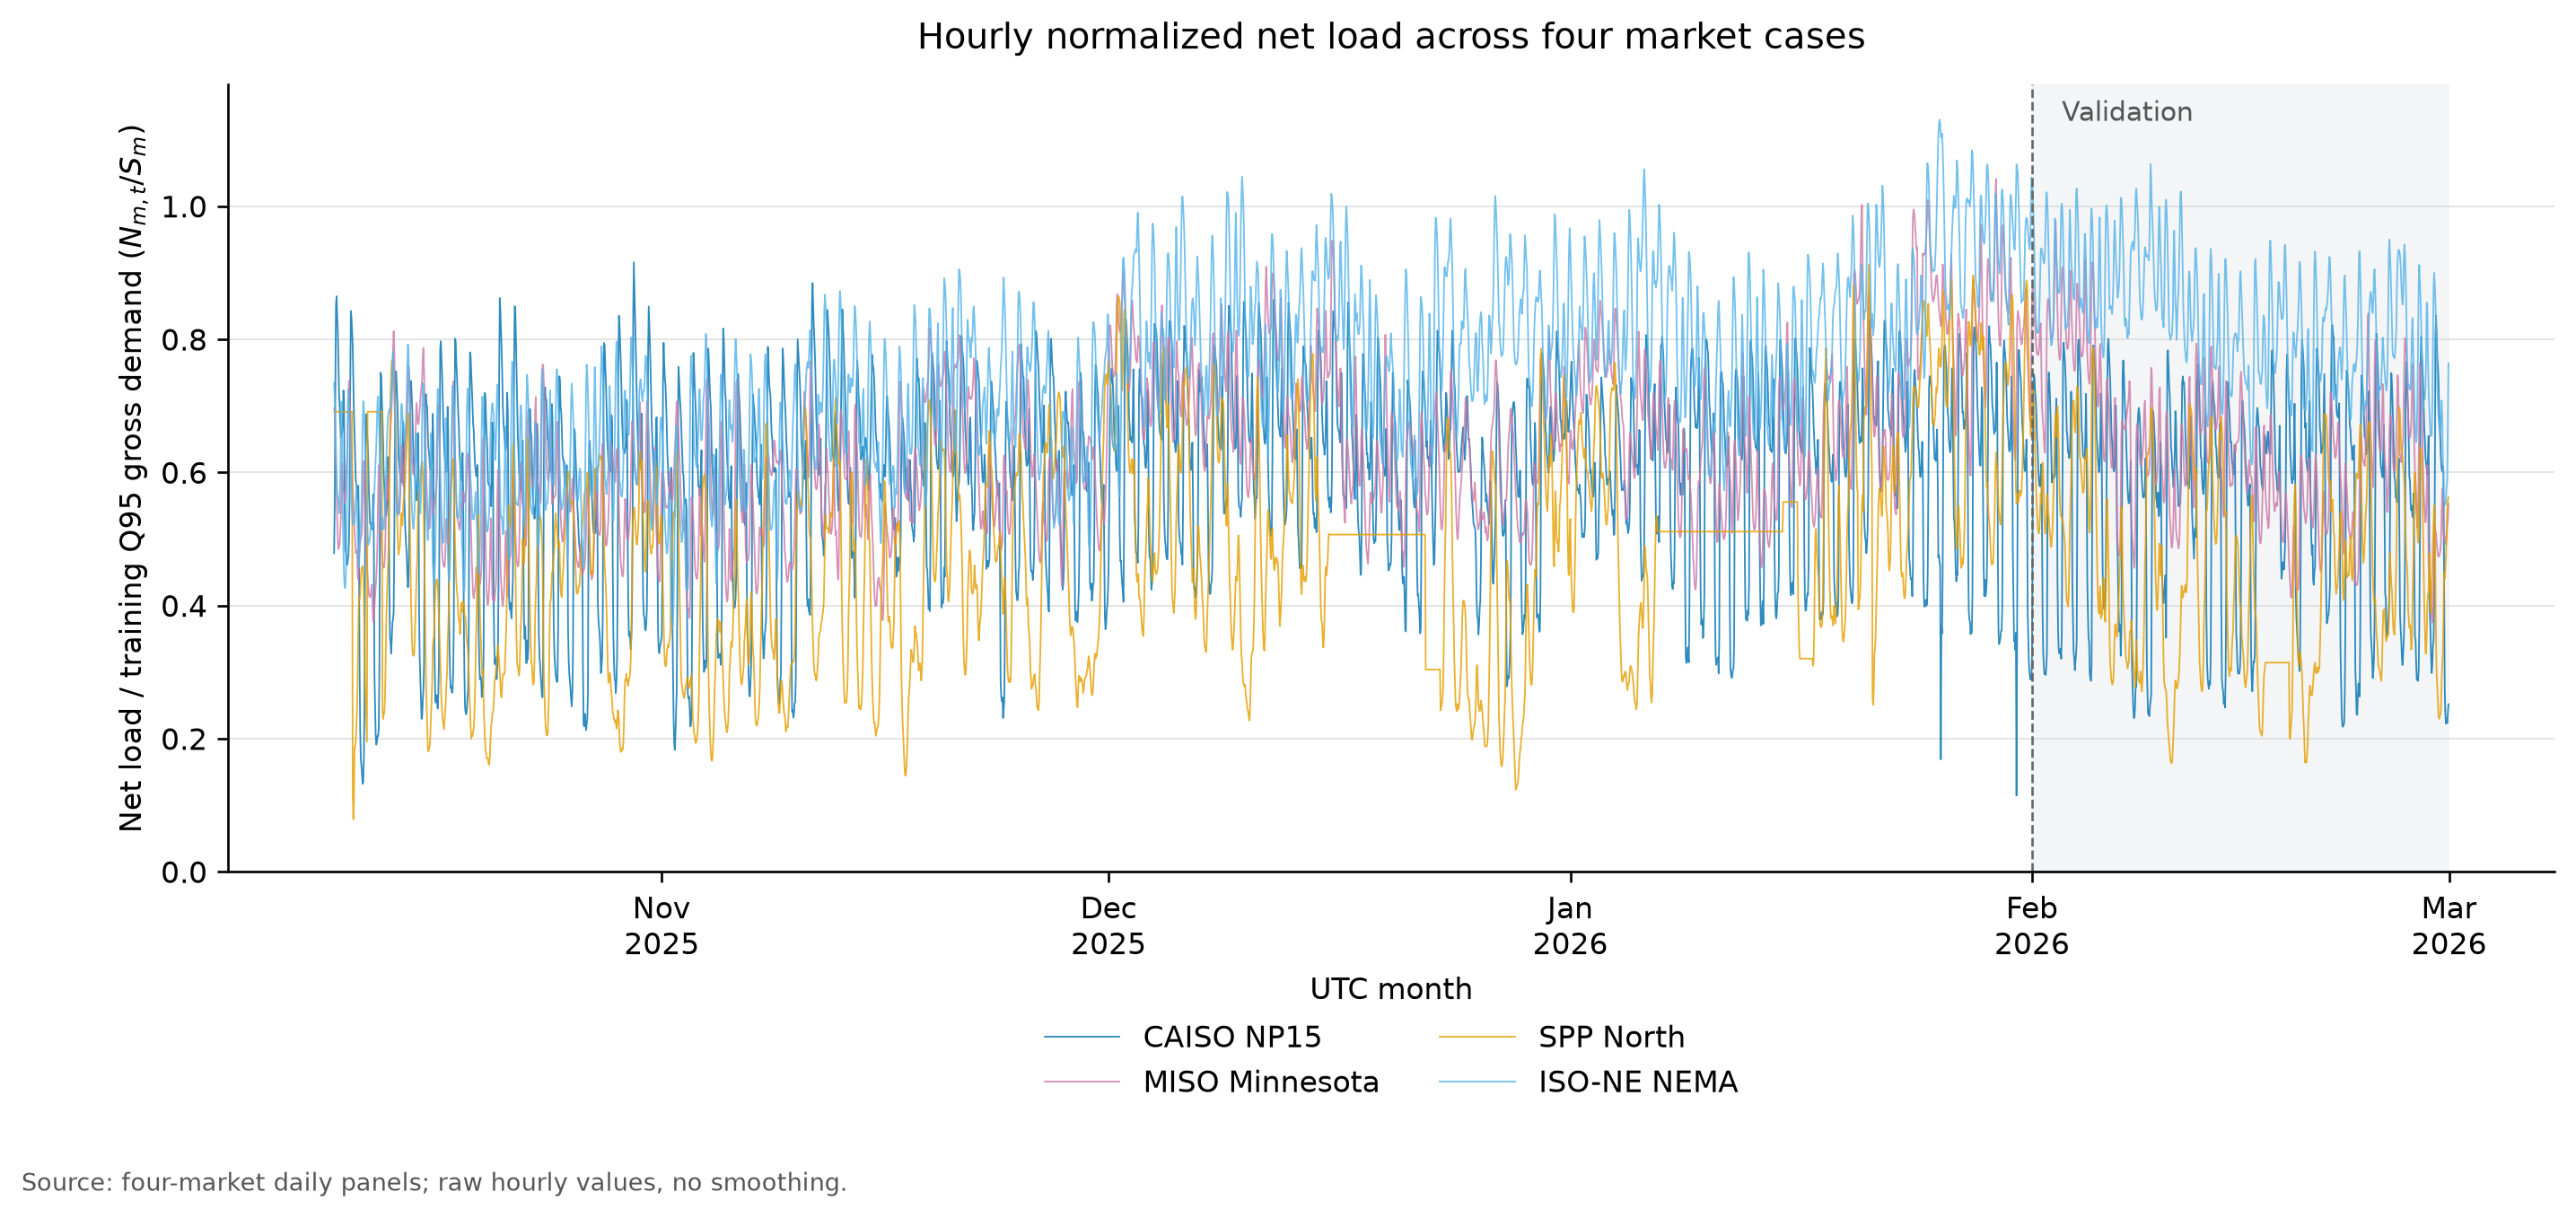
\includegraphics[width=\textwidth]{../docs/figures/four_market_v2/four_market_normalized_net_load.png}
  \caption{Hourly net load for all four active market cases on one shared axis,
  normalized by each market's training-only Q95 gross-demand scale \(S_m\).
  The figure contains 3,408 active decision hours per market from the 142
  calendar windows. Values are hourly and unsmoothed; warm and terminal-tail
  rows are not plotted.}
  \label{fig:energy-normalized-net-load}
\end{figure}

\begin{figure}[htbp]
  \centering
  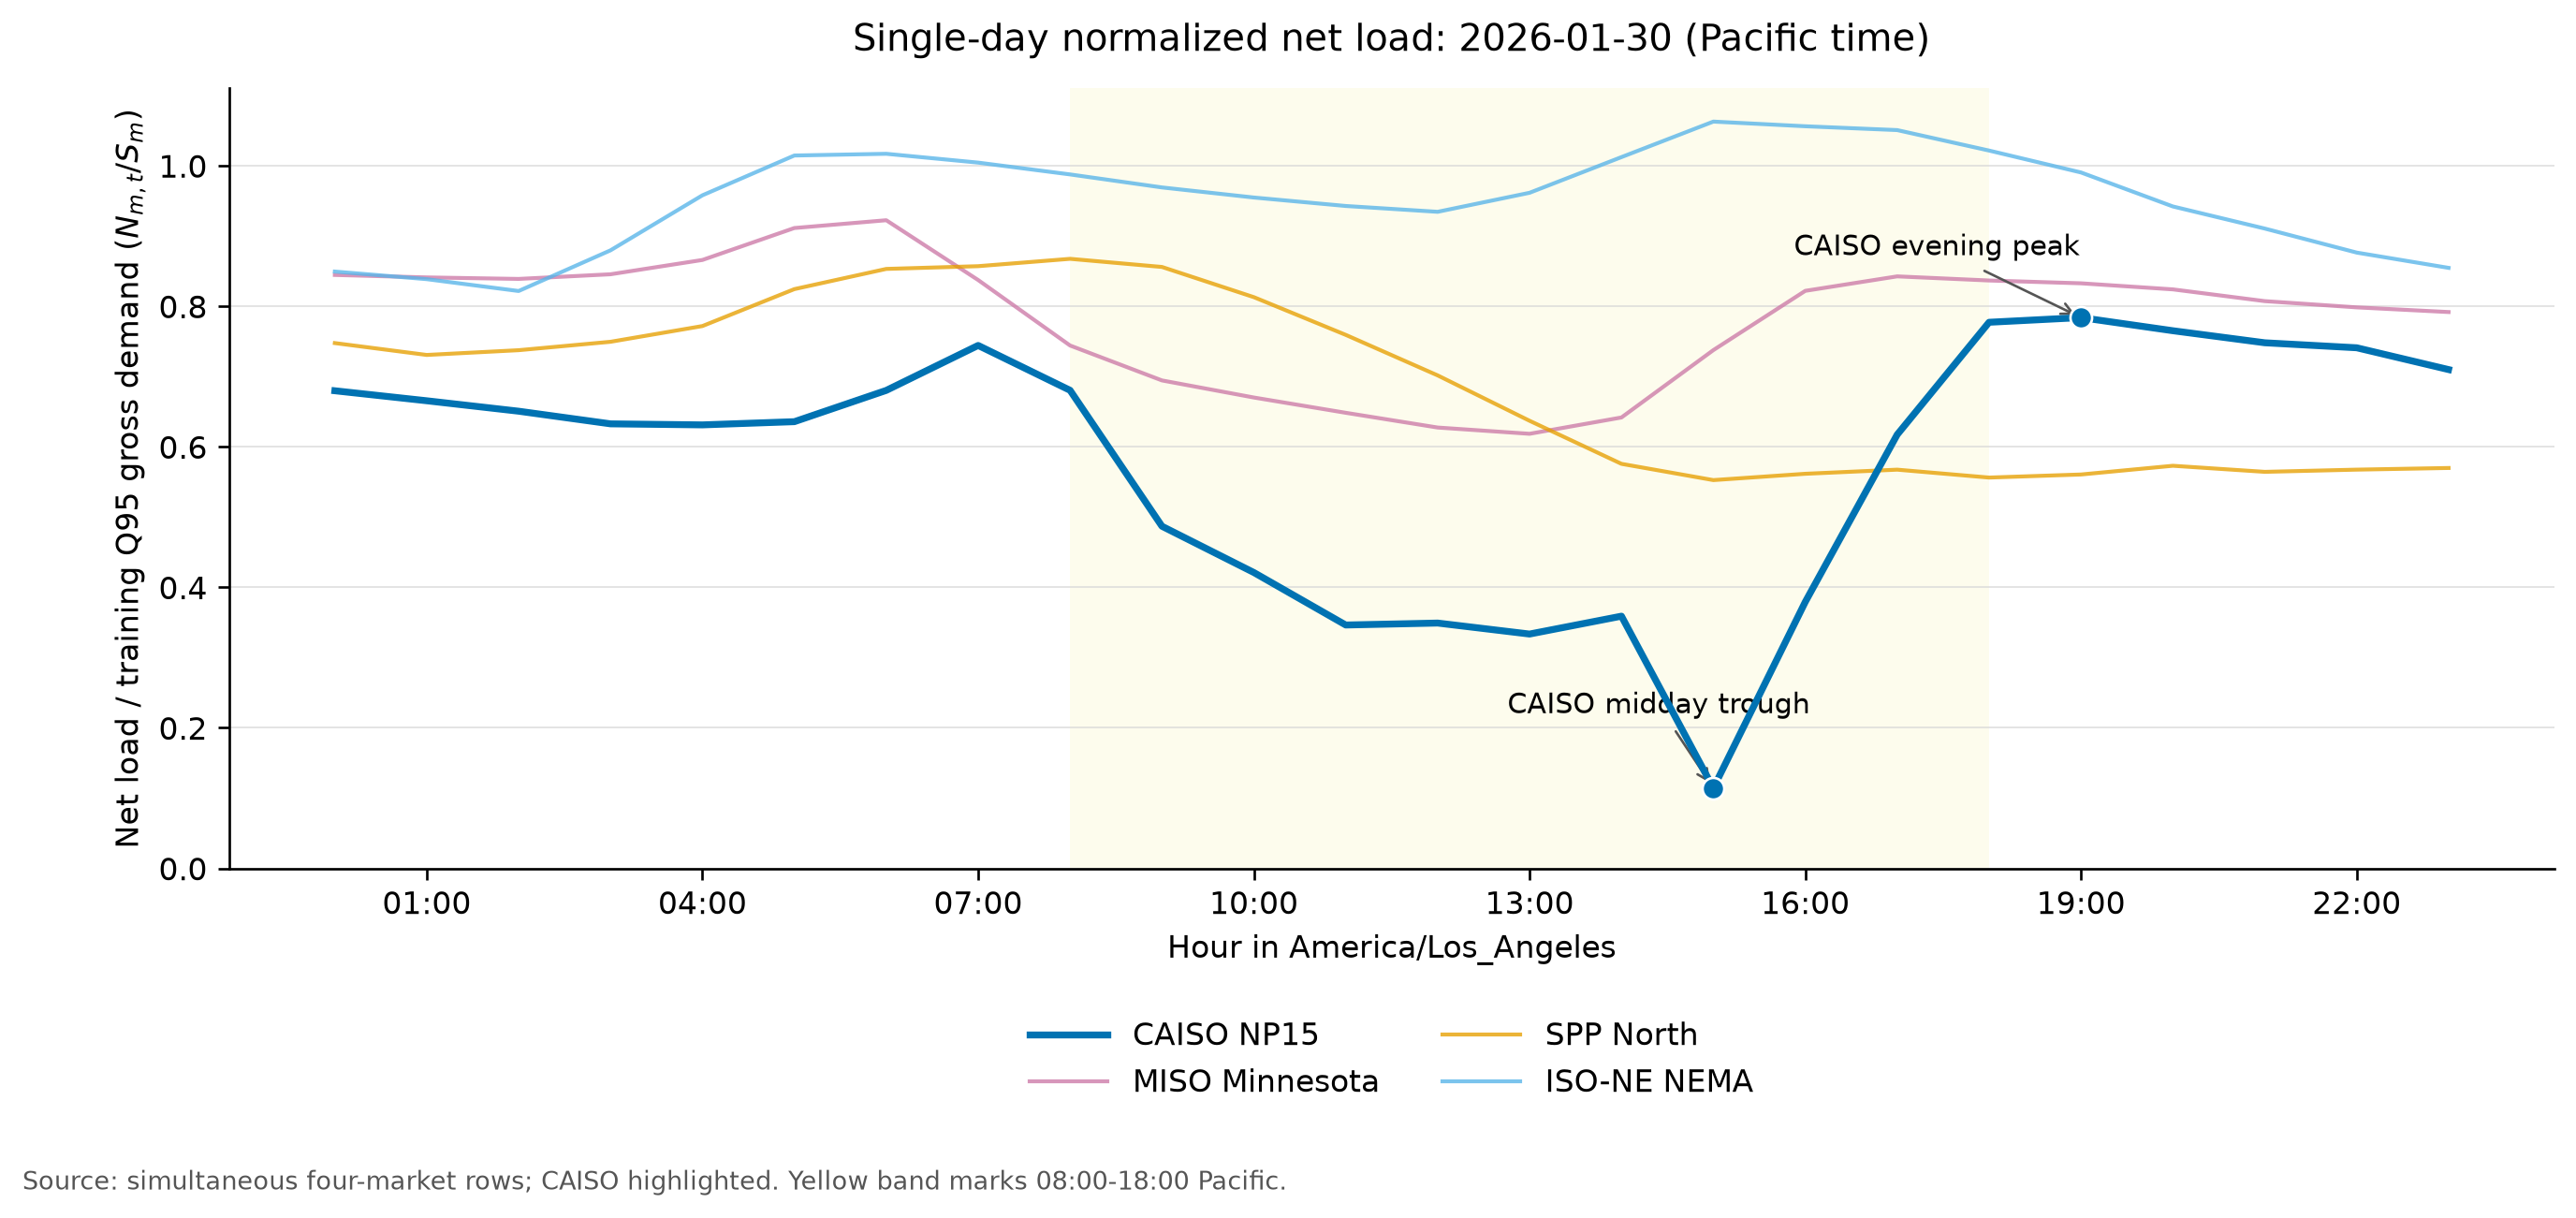
\includegraphics[width=\textwidth]{../docs/figures/four_market_v2/single_day_normalized_net_load.png}
  \caption{One-day zoom for 2026-01-30 in Pacific time. The day is selected
  deterministically from the training split as the complete CAISO day with the
  largest evening-peak minus midday-trough normalized net-load rise. CAISO is
  highlighted to expose the duck curve; the other three lines show the same
  simultaneous UTC hours on the Pacific-time axis. Values are hourly and
  unsmoothed.}
  \label{fig:energy-single-day-duck-curve}
\end{figure}

Each mapped site has a nominal 500 MW capacity. Its fitted peak proxy is
0.505\%--2.704\% of the associated market scale, as
Table~\ref{tab:energy-market-scales} shows. These realized ratios are a design
note, not a penetration gate or a model of market feedback. They support the
stated price-taking interpretation only as a small-load approximation.

\subsection{Causal forecast construction}
\label{subsec:energy-forecasts}

No operator forecast is included in the acquired source data. The repository's
forecast-construction pipeline therefore fits causal ridge models for gross
demand and net load from the observed panel. Features are observed lags at 1,
3, 24, and 168 hours; trailing means over 24 and 168 hours; and sine/cosine
encodings of target hour and day of week.

For each date in the October--January policy-learning calendar, a new
expanding-window forecast vintage is fitted, and every target used by that
vintage strictly precedes its issue date. At the 2026-02-01 boundary, the final
forecast is frozen for February validation. This forecast fitting is separate
from the PPO policy training described later: the former estimates future grid
conditions, while the latter learns how to schedule workload using those
causal estimates.

The staged forecast files contain one-hour and three-hour records. The final
factory uses the three-hour model to assemble a causal trajectory with
endpoints at \(t+1\), \(t+2\), and \(t+3\). The corresponding forecasts were
issued at \(t-2\), \(t-1\), and \(t\), respectively, so the latest issue time
never follows the scheduling-decision timestamp. A single model fitted on the
full October--February panel would leak later targets backward into earlier
decisions, so it is not used. Realized future load or real-time price is never
used as a feature. Forecast age, vintage, and quality are not policy
observations.

The resulting panel supplies the physical baseline, causal forecast state, and
price context used by the system model in
Section~\ref{sec:problem-statement}. These quantities are data inputs; the
optimization objective is defined only after the system boundary.

\subsection{Artifact and reproduction boundary}
\label{subsec:energy-reproduction}

The active data boundary is deliberately plain. \codepath{data/four_market_v2/calendar.json}
selects 114 training paths and 28 validation paths; \codepath{data/four_market_v2/frozen_stats.json}
contains the fixed training-only normalization values. The factory reads the
referenced canonical source panels rather than copying them into a second
source store. Ordinary validation checks interval completeness, duplicate rows,
units, common-calendar membership, and the required physical tuple before a
fixture is generated; it rejects incomplete native-hour aggregation and does
not forward-fill or interpolate missing observations.

The active factory and figures can be checked from the repository root:

\begin{verbatim}
python scripts\build_four_market_v2_factory.py
python scripts\run_four_market_v2_campaign.py preflight
python scripts\build_energy_thesis_figures.py
\end{verbatim}

There is one factory \codepath{output/four_market_v2/factory/factory.json} and
one set of daily \codepath{fixture.json} files. The figure builder renders
Figures~\ref{fig:energy-normalized-net-load} and
\ref{fig:energy-single-day-duck-curve} from the same calendar and source
panels. This is ordinary file-and-content validation.

\subsection{Limitations}
\label{subsec:energy-limitations}

The retained source context spans September 2025 through February 2026 and
cannot support prior-year, future-year, or long-run seasonal claims. All four physical tuples are
balancing-authority-wide EIA series, while prices are operator hubs or zones.
These geography differences do not represent local feeder conditions.

The model is price-taking: data-center actions do not change LMP, dispatch,
unit commitment, reserves, congestion, or renewable output. Day-ahead LMP is
not a retail tariff. The forecast is a reconstructed causal model rather than
an operator-issued forecast. The panel contains no carbon-intensity input, and
carbon is not optimized. A new sealed calendar, forecast freeze, and protocol
will be required after the four-market design is finalized.

\section{Experimental Transformations and Modeling Assumptions}
\label{sec:experimental-transformations}

The preceding sections describe measured source data. The remaining steps are
experimental choices: they map sources together, change temporal resolution,
assign provisional deadlines, and set facility scale. None of those choices is a
property claimed by Google, EIA, or the market operators.

\subsection{Cell-to-market mapping}
\label{subsec:transform-mapping}

\begin{table}[htbp]
  \centering
  \caption{Active four-market mapping and proxy scale.}
  \label{tab:active-market-map}
  \begin{tabular}{@{}llllr@{}}
    \toprule
    Site & Market case & Physical series & Borg cell & Rated power \\
    \midrule
    Northern California & CAISO NP15 & EIA CISO & \(a\) & 500 MW \\
    Minnesota & MISO Minnesota & EIA MISO & \(b\) & 500 MW \\
    SPP North & SPP North & EIA SWPP & \(c\) & 500 MW \\
    Boston/NEMA & ISO-NE NEMA & EIA ISNE & \(d\) & 500 MW \\
    \bottomrule
  \end{tabular}
\end{table}

The market names describe the electricity cases, not the undisclosed physical
locations of the Borg cells. Cells \(e\)--\(h\) are not mixed into the active
mapping; they remain a disjoint workload holdout for a later experiment.

\subsection{Five-minute traces to hourly arrivals}
\label{subsec:transform-hourly-workload}

Each tier curve contains 8,929 indexed samples. The final terminal boundary row
does not represent another complete five-minute interval, so it is excluded.
The remaining 8,928 samples are averaged in consecutive groups of twelve,
producing one 744-hour service profile and one 744-hour batch profile per cell.

The hourly interval is chosen to match all parts of the experiment on one
clock: day-ahead prices, the canonical EIA panel, forecasts, scheduling
decisions, and batch deadlines are hourly. Because each five-minute value is a
normalized utilization rate, its twelve-sample hourly mean represents the
average compute demand during that hour; multiplying that mean by one hour
gives the normalized compute-hours to be served. This conversion also keeps the
decision horizon tractable. Its cost is lost subhourly detail: five-minute
spikes and opportunities to move work within an hour are not modeled, so the
results support hourly scheduling claims only.

Those hourly profiles are repeated from a common 2025-09-01 UTC alignment epoch
to cover the electricity calendar. This preserves the measured within-month
shape but does not claim that May 2019 Borg work occurred contemporaneously
with 2025--2026 grid conditions. Repeating one month also suppresses long-run
growth, seasonality, and rare workload regimes.

\subsection{Coarse experimental batch deferral windows}
\label{subsec:transform-deadlines}

ClusterData2019 measures CPU use and the tier classification, but it does not
report a job's actual required completion time. The active protocol therefore
sets the four maximum batch deferral windows explicitly to
\([H_a,H_b,H_c,H_d]=[2,1,2,3]\) hours. They are provisional protocol
parameters, not derived from deleted duration statistics, Borg SLOs, or customer
commitments.

At hourly resolution, \(H_m=1\) means batch arriving in hour \(t\) must execute
within that same scheduling interval, before the \(t+1\) boundary. A two-hour
window permits execution in \(t\) or \(t+1\); a three-hour window permits any of
three consecutive hourly intervals. Thus a deadline is an inclusive number of
hourly execution opportunities, not a claim of subhour precision. The model
cannot distinguish a task that could wait ten minutes from one that could wait
fifty minutes within the same hour. This deliberately coarse semantics matches
the hourly price, grid, forecast, and decision data, while leaving five-minute
workload spikes and within-hour scheduling outside the model.

The active workload is raw: its service and batch columns are passed through
without an admission envelope, reclassification, or paired workload variant.
The largest simultaneous fleet-wide service-plus-batch arrival is
2.4244025972 normalized work units, below the total capacity of four. This
checks raw-arrival feasibility; EDF, capacity, and terminal constraints still
govern which batch work may be deferred.

\subsection{Direct 500 MW proxy rating}
\label{subsec:transform-scaling}

Each site's normalized compute capacity remains one work unit per hour, the
same scale used by the measured utilization curve. Facility power is assigned
directly:
\begin{itemize}
  \item compute capacity: \(K_c=1\) normalized work unit per hour;
  \item rated power: \(R_c=500\) MW per site; and
  \item fleet total: \(4\times500=2{,}000\) MW.
\end{itemize}

The 500 MW value is an experimental nameplate assumption, not a value disclosed
by Google. No five-times workload or compute-capacity replication is used.

\subsection{Conversion from executed work to power}
\label{subsec:transform-runtime-power}

Let \(w_{c,t}\) be service plus batch work executed at site \(c\) during hour
\(t\), and let \(K_c=1\) be site compute capacity. Runtime utilization is
\(w_{c,t}/K_c\), bounded to the fitted range \([0,1]\). The corresponding proxy
power is
\begin{equation}
  P_{c,t}
  =
  500
  \left(
    \alpha_c + \beta_c \frac{w_{c,t}}{K_c}
  \right)
  \text{ MW},
  \label{eq:transform-runtime-power}
\end{equation}
using the cell-specific PowerData2019 coefficients from
Table~\ref{tab:powerdata-coefficients}. The 500 MW rating is an experimental
facility scale; PowerData2019 provides only the normalized power relationship.
Because \(\alpha_c+\beta_c<1\), fitted full-utilization power is approximately
434, 462, 483, and 476 MW for cells \(a\)--\(d\), respectively. The model does
not renormalize those measured fits merely to force 500 MW at full utilization.

The repeated measured aggregate profile supplies three hours of warm power at
the start of each episode. Once decisions begin, power is recomputed from the
work actually routed and executed; it is not a fixed replay of the measured
profile.

\subsection{Active factory boundary}
\label{subsec:transform-factory}

The transformation is implemented in \codepath{energy_model_v3/four_market_v2.py}
and governed by the single protocol
\codepath{env/protocols/four_market_v2.yaml}. There is one factory descriptor,
\codepath{output/four_market_v2/factory/factory.json}, and one fixture set under
\codepath{output/four_market_v2/factory/windows}. The factory uses
\codepath{data/four_market_v2/calendar.json} to select 114 randomized training
windows and the named, exact 28-window February validation set. It has no test
split.

The factory references the selected canonical source panels rather than copying
them. For each daily window it generates a \codepath{fixture.json} containing
the raw hourly workload arrivals, deadlines, warm power history, and site
parameters; its corresponding factory record supplies the canonical-panel
reference. An episode has three warm hours, 24 active decision hours, and a
three-hour terminal tail. The factory builder constructs the selected fixtures;
preflight validates their ordinary structural, capacity, calendar, and
causal-boundary conditions before a campaign uses them. There are no parallel
factories or alternate workload variants.

\section{Problem Statement and System Boundary}
\label{sec:problem-statement}

\subsection{Purpose of the system model}
\label{subsec:problem-purpose}

Sections~\ref{sec:clusterdata2019}--\ref{sec:energy-data} describe the source
data and fitted power model. Section~\ref{sec:experimental-transformations}
defines how those sources become the active experiment. Together they provide
the fixed inputs to the scheduling problem defined here. This section does not
yet choose an optimization algorithm; it identifies:
\begin{enumerate}
  \item what is fixed and observed;
  \item what an operator is allowed to change;
  \item which outcomes are physically or operationally infeasible; and
  \item which real-world effects are outside the modeled boundary.
\end{enumerate}

The mathematical objective, reward, and PPO implementation are introduced only
after this feasible system boundary, in
Section~\ref{sec:optimization-objective}.

\subsection{Sets, time, and fixed inputs}
\label{subsec:problem-given-inputs}

Let \(\mathcal{M}=\{1,\ldots,4\}\) denote the four proxy data-center sites and
their one-to-one electricity-market cases from
Table~\ref{tab:active-market-map}. A site and its attached market share
the same index \(m\). Let \(t\) denote an hourly decision.

\begin{longtable}{@{}L{0.27\textwidth}L{0.31\textwidth}L{0.34\textwidth}@{}}
  \caption{Quantities treated as given by the system model.}
  \label{tab:problem-given-inputs}\\
  \toprule
  Given quantity & Source & Role in the problem \\
  \midrule
  \endfirsthead
  \toprule
  Given quantity & Source & Role in the problem \\
  \midrule
  \endhead
  Hourly service arrivals \(s_{m,t}\)
    & \codepath{data/cells/cell_X_tiers.csv};
      Section~\ref{subsec:clusterdata-tier-split}
    & Work that must be completed during its arrival hour. \\
  Hourly batch arrivals \(q_{m,t}\)
    & Same raw measured tier curves
    & Work that may wait and move, but must finish by its assigned provisional
      deadline. \\
  Batch deadline \(H_m\)
    & \codepath{env/protocols/four_market_v2.yaml};
      Section~\ref{subsec:transform-deadlines}
    & Explicit provisional maximum hourly deferral horizon for arrivals
      associated with cell \(m\). \\
  Compute capacity \(K_m\)
    & Active v2 protocols
    & Maximum service plus batch work executable at site \(m\) in one hour;
      \(K_m=1\) in the active design. \\
  Rated power and affine coefficients
    & Active protocol and \codepath{data/power_model_params.json};
      Equation~\eqref{eq:transform-runtime-power}
    & Converts executed work at a destination site into market-level MW. \\
  Net load \(N_{m,t}\), gross demand, wind, and solar
    & Canonical energy panel; Sections~\ref{subsec:energy-canonical} and
      \ref{subsec:energy-net-load}
    & Defines the exogenous physical grid trajectory before modeled fleet power. \\
  Day-ahead LMP \(L^{\mathrm{DA}}_{m,t}\)
    & Canonical price panel; Table~\ref{tab:energy-sources}
    & Supplies wholesale economic context and a post-hoc cost comparison. \\
  Causal forecast trajectory
    & Active canonical panel;
      Section~\ref{subsec:energy-forecasts}
    & Provides estimates of upcoming gross and net load available at decision
      time. \\
  Training-only scales and normalizers
    & \codepath{data/four_market_v2/frozen_stats.json};
      Equation~\eqref{eq:energy-market-scale}
    & Makes market states and later ramp comparisons commensurate without using
      February validation data. \\
  Three-hour warm power history
    & Active daily fixtures;
      \codepath{energy_model_v3/four_market_v2.py}
    & Supplies modeled preceding fleet power, derived from raw warm arrivals, for
      the first 1 h and 3 h ramp windows of each daily episode. \\
  \bottomrule
\end{longtable}

The authoritative assembly of these inputs is recorded in the single
\codepath{output/four_market_v2/factory/factory.json}. Each generated daily
fixture contains the required site parameters, raw service and batch arrivals,
deadline horizons, and warm power; its factory record references the canonical
market panel. The factory uses ordinary validation.

\subsection{Proxy-fleet interpretation}
\label{subsec:problem-proxy-fleet}

The four sites are controlled archetypes, not identified Google facilities and
not claims about the undisclosed geography of the Borg cells. Each active
site has:
\begin{itemize}
  \item normalized compute capacity \(K_m=1\);
  \item proxy rated power \(R_m=500\) MW;
  \item one ClusterData2019 workload profile;
  \item one PowerData2019 affine power model; and
  \item one attached electricity-market case.
\end{itemize}

The active fleet is therefore 2 GW. Assigning work to site \(m\) determines
the power added to market \(m\) through
Equation~\eqref{eq:transform-runtime-power}. The workload shape and power
response are measured or fitted; the 500 MW magnitude and the cell-to-market
pairing are experimental assumptions.

All compute work is represented as divisible aggregate work. Individual jobs,
applications, users, machine types, and task placement inside a cell are not
modeled. Memory appears only in a diagnostic PowerData fit and is not a runtime
resource constraint.

\subsection{Controllable decisions}
\label{subsec:problem-decisions}

At each hour, a feasible scheduler may control three quantities:
\begin{enumerate}
  \item \textbf{Service destination.} It chooses how the fleet-wide total of
        immediate service is divided among the four sites.
  \item \textbf{Batch execution volume.} It chooses how much queued batch work
        to execute now rather than retain for a later hour.
  \item \textbf{Batch destination.} It chooses where the selected batch work is
        executed.
\end{enumerate}

Let \(x^{\mathrm{svc}}_{m,t}\) and
\(x^{\mathrm{bat}}_{m,t}\) denote service and batch work executed at destination
site \(m\). Let \(z_t=\sum_m x^{\mathrm{bat}}_{m,t}\) be total batch execution.
The origin of service is not retained after arrivals are pooled. Batch origin
is retained in the deadline ledger, and an exact transport matrix
\(\Pi_{i,j,t}\) accounts for movement from origin \(i\) to execution site \(j\).

These are operational decisions, not yet PPO actions. The 9-dimensional
preference interface described later is one attempted parameterization of this
three-part decision.

\subsection{Immediate-service and batch semantics}
\label{subsec:problem-workload-semantics}

Immediate service cannot be delayed:
\begin{equation}
  \sum_{m \in \mathcal{M}} x^{\mathrm{svc}}_{m,t}
  =
  \sum_{m \in \mathcal{M}} s_{m,t}.
  \label{eq:problem-service-conservation}
\end{equation}

Batch work enters a global earliest-deadline-first (EDF) queue while retaining
its origin and absolute deadline. If \(Q_t\) is queued mass before new
execution, aggregate queue accounting follows
\begin{equation}
  Q_{t+1}
  =
  Q_t
  +
  \sum_m q_{m,t}
  -
  z_t.
  \label{eq:problem-batch-ledger}
\end{equation}

The queue must conserve mass exactly, work due by a deadline must be executed
no later than that deadline, and all admitted batch work must be complete at
the episode terminal. The implementation is the
\codepath{EDFQueue} ledger in \codepath{env/ramp_v6/models.py}.

The raw measured service and batch columns are the current problem instance.
No arrival cap reclassifies batch work as immediate service.

\subsection{Capacity and transport feasibility}
\label{subsec:problem-feasibility}

Executed work cannot exceed destination capacity:
\begin{equation}
  0
  \leq
  x^{\mathrm{svc}}_{m,t}
  +
  x^{\mathrm{bat}}_{m,t}
  \leq
  K_m
  \qquad
  \forall m,t.
  \label{eq:problem-site-capacity}
\end{equation}

For batch work drained from origin \(i\), transport accounting requires
\begin{align}
  \sum_j \Pi_{i,j,t}
    &= o_{i,t}, \\
  \sum_i \Pi_{i,j,t}
    &= x^{\mathrm{bat}}_{j,t},
  \label{eq:problem-transport}
\end{align}
where \(o_{i,t}\) is the EDF-selected batch amount from origin \(i\). This
matrix enforces conservation only. It is not a network-flow model.

Routing is otherwise unrestricted. The decoder nevertheless calculates a
conservative future-batch capacity requirement from the data-derived raw batch
arrivals and their provisional deadlines, reserving capacity needed to make the
EDF ledger feasible. It does not use grid forecasts to waive a deadline.

The model imposes no latency, wide-area bandwidth, data-residency,
transfer-energy, replication, or movement-cost constraint. Consequently,
spatial flexibility is an optimistic upper bound on what a real operator could
use.

\subsection{Episode and terminal boundary}
\label{subsec:problem-episode}

Each episode represents one UTC day with:
\begin{itemize}
  \item three preceding canonical-panel hours for ramp history;
  \item 24 active arrival and decision hours; and
  \item a three-hour terminal tail with no new arrivals.
\end{itemize}

The tail allows late-day batch work to finish and allows 1 h and 3 h windows
ending after the final arrival hour to be scored. Circular wrap to the start of
the day is forbidden. The batch queue starts empty at reset and must be empty
at the true terminal. These rules are generated in
\codepath{energy_model_v3/four_market_v2.py} and enforced by
\codepath{env/ramp_v6/environment.py}.

\subsection{Causal information boundary}
\label{subsec:problem-causality}

A decision at hour \(t\) may depend only on information available by \(t\):
\begin{itemize}
  \item current and three trailing hours of observed gross and net load;
  \item native 1 h and 3 h ramps that have already closed;
  \item forecast endpoints whose issue time is no later than \(t\);
  \item current service and batch arrivals, queued work, and deadlines;
  \item previous modeled site power;
  \item current day-ahead LMP; and
  \item hour, day-of-week, and episode-progress features.
\end{itemize}

Realized future load, realized future real-time price, and forecasts issued
after \(t\) are prohibited. Formally, a scheduling rule \(\mu_t\) must be a
function only of the causal information set \(\mathcal{I}_t\):
\begin{equation}
  \left(
    x^{\mathrm{svc}}_t,
    z_t,
    x^{\mathrm{bat}}_t
  \right)
  =
  \mu_t(\mathcal{I}_t).
  \label{eq:problem-causal-policy}
\end{equation}

\subsection{Grid and market boundary}
\label{subsec:problem-grid-boundary}

The four physical net-load trajectories and day-ahead prices are exogenous. The
modeled fleet is price-taking and does not alter dispatch, LMP, renewable
generation, unit commitment, reserves, congestion, or the source forecasts.
Fleet power is added to native net load for counterfactual evaluation, but the
source grid trajectory itself is unchanged.

The price-taking approximation is an experimental caveat, not a penetration
gate or a simulated market response. The realized fitted peak/site-scale ratios
are 0.505\%--2.704\%, but market-level net load still does not represent the
local substation, feeder, nodal constraint, or utility tariff faced by a real
facility.

\subsection{Three comparison systems}
\label{subsec:problem-baselines}

The thesis distinguishes three systems:
\begin{enumerate}
  \item \textbf{Native grid.} \(N_{m,t}\) without any modeled data-center power.
        This is a physical counterfactual, not an operating policy.
  \item \textbf{Operational status quo.} Native grid plus fleet power from an
        evaluation-only baseline that routes service and batch in origin
        proportions and requests immediate batch drainage under the same
        capacity, conservation, and deadline rules. It maintains an independent
        shadow queue.
  \item \textbf{Candidate policy.} Native grid plus fleet power produced by the
        learned routing and timing preferences under those same feasibility
        rules.
\end{enumerate}

Status quo and candidate use identical market, workload, forecast, capacity,
and deadline windows. The independent shadow queue and baseline action are
implemented by \codepath{_status_quo_action} in
\codepath{env/ramp_v6/environment.py}; evaluation aggregation is implemented in
\codepath{ramp_rl/evaluation.py}.

The native comparison isolates whether the modeled fleet increases or decreases
the grid's pre-existing ramp. The status-quo comparison asks the more
operational question: whether the candidate schedule improves on a simple
grid-unaware way of running the same fleet.

\subsection{Problem statement}
\label{subsec:problem-formal-statement}

The scheduling cases span many energy dates to avoid designing against one
unusually favorable grid day or month. They do not contain many independent
months of workload: one measured May 2019 Borg profile is repeated while net
load, renewable output, day-ahead price, and causal forecasts change. The 114
October--January days supply varied conditions for learning a schedule; the 28
later February days assess it on unseen energy dates. The separate cells
\(e\)--\(h\) holdout would assess transfer to unseen workload and is outside the
current experiment.

\begin{quote}
\textbf{Problem statement.}
Given four hourly raw service and batch arrival streams, provisional batch
deadlines, four capacity and power models, causal physical-grid and forecast
information, and day-ahead prices, construct a causal hourly schedule for
service destination, batch execution volume, and batch destination such that:
\begin{enumerate}
  \item all immediate service is completed in its arrival hour;
  \item all batch work is conserved and completed by its deadline;
  \item no site exceeds compute capacity and the terminal queue is empty; and
  \item the fleet's added power reduces, or at minimum does not amplify, the
        native grid's rapid net-load changes across the four market cases.
\end{enumerate}
\end{quote}

This statement does not prescribe reinforcement learning, a neural policy, the
1 h/3 h weights, or a scalar reward. Those choices constitute the attempted
solution defined next. Day-ahead cost remains a post-hoc outcome for comparing
policy and status quo, not a feasibility constraint or problem-statement gate.

\section{Optimization Objective and Policy Inputs}
\label{sec:optimization-objective}

\noindent
Within the feasible system defined in Section~\ref{sec:problem-statement}, the
active four-market design chooses a pure ramp objective, policy representation,
and constraint decoder. This section therefore describes the attempted solution,
not an additional data source or a restatement of the problem.

\subsection{What is decided each hour}
\label{subsec:objective-hourly-decision}

Each episode advances in one-hour decisions. At hour \(t\), the policy emits
9 preferences for the four-site fleet:
\begin{enumerate}
  \item four preferences for the destination of immediate service work;
  \item one preference for how much queued batch work to execute; and
  \item four preferences for the destination of that batch work.
\end{enumerate}

The policy does not directly set MW. A constraint-only decoder converts the
preferences into feasible service and batch allocations, enforcing immediate
service completion, site capacity, earliest-deadline-first batch requirements,
and exact work conservation. The PowerData2019 model then converts executed
work at each site into market-level data-center power \(P_{m,t}\).

Only after \(P_{m,t}\) is known does the environment score ramp windows whose
right endpoint is hour \(t\). Every reward therefore uses the action just
executed and already observed past values; no future realized load enters the
score.

\subsection{Meaning of the 1 h and 3 h horizons}
\label{subsec:objective-horizons}

The horizon \(h\) is the distance between the two endpoints of a ramp:
\begin{itemize}
  \item \(h=1\) compares hour \(t\) with hour \(t-1\), capturing a fast
        hour-to-hour change; and
  \item \(h=3\) compares hour \(t\) with hour \(t-3\), capturing a broader
        multi-hour rise or fall.
\end{itemize}

Dividing by \(h\) expresses both as an average change per hour, so the two
horizons are comparable. The objective gives 40\% weight to the 1 h horizon
and 60\% to the 3 h horizon. This favors sustained multi-hour smoothing while
still penalizing sharp hourly changes.

These horizons are experimental choices rather than universal grid constants.
One hour matches the scheduling and source-data resolution. Three hours matches
the longest batch deadline, the causal forecast trajectory, and the window over
which an evening renewable decline can become a sustained ramp. Using both
prevents a schedule from smoothing a single hour while merely shifting the
change into the next few hours. The 40/60 weights place more emphasis on that
sustained effect and should ultimately be tested by sensitivity analysis.

\subsection{Native and data-center-adjusted ramps}
\label{subsec:objective-native-adjusted}

Let \(N_{m,t}\) be the physical net load in market \(m\) before adding the
modeled fleet, \(P_{m,t}\) the fleet power assigned to that market, and \(S_m\)
the training-only Q95 gross-demand scale from
Equation~\eqref{eq:energy-market-scale}. The two normalized ramps are
\begin{align}
  b_{m,t,h}
    &= \frac{N_{m,t}-N_{m,t-h}}{S_m h}, \\
  a_{m,t,h}
    &= \frac{(N_{m,t}+P_{m,t})-(N_{m,t-h}+P_{m,t-h})}{S_m h}.
  \label{eq:energy-ramps}
\end{align}

The native ramp \(b_{m,t,h}\) answers: ``How quickly was the grid already
changing without this modeled fleet?'' The adjusted ramp \(a_{m,t,h}\)
answers: ``How quickly would net load change after adding the fleet schedule?''
Normalization by \(S_m\) prevents a large market such as MISO from dominating
a smaller market such as ISO-NE solely because its MW scale is larger.

The target is the ramp of the combined grid-facing trajectory \(N+P\), not the
ramp of data-center power \(P\) alone. There is no term that minimizes
\(\lvert P_{m,t}-P_{m,t-h}\rvert\). A sharp decrease in data-center power during
an upward native-grid ramp, or a sharp increase during a downward native-grid
ramp, can be beneficial because the two changes counteract each other. Constant
data-center power is ramp-neutral rather than automatically optimal.

The adjusted ramps are used twice. First, they are reported as physical
per-market ramp magnitudes. Second, they are compared with the native ramps to
calculate the schedule's incremental effect.

\subsection{Why ramps are squared}
\label{subsec:objective-squared-ramp}

The squared native ramp \(b_{m,t,h}^2\) is a dimensionless stress proxy for the
grid change that would have occurred without the modeled fleet. Squaring serves
two purposes:
\begin{enumerate}
  \item upward and downward ramps receive the same sign-independent burden; and
  \item a large ramp is penalized more strongly than several small ramps.
\end{enumerate}

The study does not minimize \(b^2\) itself because the modeled fleet did not cause
the underlying grid ramp. Instead, \(b^2\) is the counterfactual baseline
subtracted from the adjusted squared ramp.

Squared ramp is not directly equivalent to monetary cost. It has normalized,
dimensionless squared units and is used only as a convex severity proxy.
Real ramping cost depends on which generators respond, startup and fuel costs,
reserve requirements, congestion, and operating constraints that are outside
the model. Day-ahead LMP therefore remains a separate wholesale-cost measure;
the experiment does not convert ramp impact into dollars.

\subsection{Per-window incremental impact and PPO reward}
\label{subsec:objective-incremental-impact}

For one market, one endpoint, and one horizon, the incremental impact is
\begin{equation}
  I_{m,t,h}=a_{m,t,h}^2-b_{m,t,h}^2.
  \label{eq:energy-incremental-impact}
\end{equation}
A negative value means fleet power reduced the squared native ramp, zero is
ramp-neutral, and a positive value worsened it. The active impact at hour
\(t\) is the equal-market mean of the two weighted horizons:
\begin{equation}
  \overline{I}_t=
  \frac{1}{4}\sum_{m=1}^{4}
  \left(0.40I_{m,t,1}+0.60I_{m,t,3}\right).
  \label{eq:objective-primary-impact}
\end{equation}
The pure PPO reward is exactly
\begin{equation}
  r_t=-\overline{I}_t.
  \label{eq:objective-ramp-reward}
\end{equation}
Squaring in Equation~\eqref{eq:energy-incremental-impact} already weights large
ramps more heavily while treating upward and downward changes symmetrically.
PPO receives this scalar after the executed hourly action, so its learned
routing and timing preferences are rewarded only for making the incremental
impact more negative. There is no Lagrangian, constraint-violation penalty,
cost term, or separate terminal-tail reward: feasibility is enforced by the
decoder, and the no-arrival terminal-tail steps use this same scalar reward.

\subsection{Purpose of day-ahead energy cost}
\label{subsec:objective-energy-cost}

Day-ahead cost is a post-hoc outcome, not a reward component or pass/fail
constraint. It is calculated for the policy and status quo on identical hours:
\begin{align}
  C_{m,t}&=L^{\mathrm{DA}}_{m,t}P_{m,t}(1\ \mathrm{hour}), \\
  C_t&=\sum_{m=1}^{4}C_{m,t}, \qquad
  \rho_C=\frac{\sum_t C_t^{\mathrm{policy}}}
                 {\sum_t C_t^{\mathrm{status\ quo}}}.
  \label{eq:energy-cost}
\end{align}
Here \(L^{\mathrm{DA}}\) is USD/MWh and \(P\) is MW. The ratio describes the
wholesale cost consequence of a policy relative to the same fleet under status
quo; it does not alter training or constitute a feasibility condition.
It remains a wholesale proxy, excluding retail rates, demand charges, taxes,
ratchets, and contractual terms.

\subsection{How observations affect policy behavior}
\label{subsec:objective-observations}

Observations do not mechanically force an action. They are inputs to the PPO
network from which it learns the nine preferences described above. The active
observation vector has exactly 100 entries, counted in
Table~\ref{tab:objective-observations}. It deliberately retains causal market,
site, queue, and time state while excluding fixed site constants, forecast age,
vintage, quality metadata, and forecast bins beyond three hours.

\begin{longtable}{@{}L{0.29\textwidth}rL{0.53\textwidth}@{}}
  \caption{The exactly 100 retained observations and their decision roles.}
  \label{tab:objective-observations}\\
  \toprule
  Observation family & Count & Scheduling information it provides \\
  \midrule
  \endfirsthead
  \toprule
  Observation family & Count & Scheduling information it provides \\
  \midrule
  \endhead
  Current plus three lags of gross and net load, for four markets
    & 32 & Locates each market in its recent physical demand and residual-load
      trajectory. \\
  Native 1 h and 3 h ramps, for four markets
    & 8 & Indicates the already observed direction and rate of grid change. \\
  Causal gross/net forecasts at \(t+1,t+2,t+3\), plus a maximum-up summary
  for each trajectory and market
    & 32 & Lets the policy anticipate a forecast rise or valley without observing
      realized future load. \\
  Current day-ahead LMP, for four markets
    & 4 & Supplies known wholesale economic context; it does not enter reward or
      create a cost constraint. \\
  Service arrival, batch arrival, queued batch, and previous power, for four
  sites
    & 16 & Describes available work, backlog, and the data-center power state that
      enters the next ramp calculation. \\
  Fleet EDF urgency: work due within at most 1 h and 3 h
    & 2 & Summarizes near-term queue pressure and the need to retain feasible
      batch capacity. \\
  Episode progress, terminal-tail state, hour sine/cosine, and day-of-week
  sine/cosine
    & 6 & Identifies the recurring hourly context and approach to the terminal
      boundary. \\
  \midrule
  \textbf{Total} & \textbf{100} & \\
  \bottomrule
\end{longtable}

The forecast affects action choice, not reward calculation. Reward is computed
when a ramp window closes from realized net load and executed fleet power; this
separation permits anticipatory control without leaking future realized values.
Fixed site parameters are already part of the factory, quality and forecast-age
fields do not describe a decision-relevant changing state here, and bins beyond
three hours are intentionally outside the protocol horizon.

\section{Ten-Seed Validation Campaign and Results}
\label{sec:campaign}

Seeds 4101--4110 each request 2,000,000 interactions. All ten complete
uninterrupted (\codepath{resumed_from_interactions=0}); the safe rollout and
complete-episode boundary give 2,045,952 effective interactions per seed. All
seeds train on the same 114 calendar-selected October--January windows and
evaluate on the exact same named 28 February validation windows. The protocol,
raw workload, factory, observations, reward, and comparator are unchanged
across seeds. Cells \(e\)--\(h\) and any test calendar are not accessed.

Policy and status quo are paired within each optimizer seed, making the
optimizer seed (\(n=10\)), rather than individual hours or days, the statistical
unit. The primary paired outcome is policy minus status-quo mean incremental
ramp impact. The analysis uses an exact two-sided Wilcoxon signed-rank test,
explicitly not a t-test. Matched-pairs rank-biserial correlation is oriented so
that a positive value favors the policy. The summary also reports the
Hodges--Lehmann paired shift and 95\% seed-bootstrap intervals from 10,000
resamples.

\subsection{Overall paired result}
\label{subsec:campaign-overall}

All ten paired differences are negative: every trained policy has lower mean
incremental ramp impact than status quo on the same 28 validation days. The
policy's mean native-relative impact is
\(-7.2618\times10^{-5}\), compared with
\(-6.4573\times10^{-6}\) for status quo. The mean additional policy improvement
is therefore \(-6.6161\times10^{-5}\).

\begin{table}[htbp]
  \centering
  \small
  \caption{Locked ten-seed February validation result. Negative impact and
  negative policy-minus-status-quo differences are improvements.}
  \label{tab:ten-seed-result}
  \begin{tabular}{@{}lr@{}}
    \toprule
    Quantity & Result \\
    \midrule
    Policy mean native-relative impact & \(-7.2618\times10^{-5}\) \\
    Status-quo mean native-relative impact & \(-6.4573\times10^{-6}\) \\
    Mean paired difference & \(-6.6161\times10^{-5}\) \\
    Mean-difference 95\% seed-bootstrap interval
      & \([-6.6486,-6.5861]\times10^{-5}\) \\
    Hodges--Lehmann paired shift & \(-6.6084\times10^{-5}\) \\
    Hodges--Lehmann 95\% seed-bootstrap interval
      & \([-6.6472,-6.5679]\times10^{-5}\) \\
    Exact two-sided Wilcoxon \(p\) & \(0.001953125\) \\
    Matched-pairs rank-biserial correlation & \(1.0\) \\
    Seeds favoring policy & \(10/10\) \\
    \bottomrule
  \end{tabular}
\end{table}

With ten nonzero differences of the same sign, \(0.001953125\) is the minimum
possible two-sided exact Wilcoxon \(p\)-value for \(n=10\). Rank-biserial
correlation and the common-language seed-win effect are both 1.0. These results
show a stable optimizer-seed-level macro advantage on the fixed February
validation calendar. They do not establish transfer to cells \(e\)--\(h\), a
new year, or a sealed test calendar.

\subsection{Market heterogeneity}
\label{subsec:campaign-markets}

The macro result is not uniform across markets.
Table~\ref{tab:ten-seed-markets} reports equal-seed means. PPO beats status quo
in all ten seeds for CAISO, SPP, and ISO-NE, but in zero of ten for MISO.

\begin{table}[htbp]
  \centering
  \small
  \caption{Per-market mean incremental impact across ten optimizer seeds.}
  \label{tab:ten-seed-markets}
  \begin{tabular}{@{}lrrrr@{}}
    \toprule
    Market & Policy & Status quo & Policy minus status quo & Wins \\
    \midrule
    CAISO NP15
      & \(-1.0951\times10^{-4}\) & \(-8.8483\times10^{-6}\)
      & \(-1.0067\times10^{-4}\) & \(10/10\) \\
    MISO Minnesota
      & \( 2.8800\times10^{-7}\) & \(-4.8263\times10^{-6}\)
      & \( 5.1143\times10^{-6}\) & \(0/10\) \\
    SPP North
      & \(-2.2077\times10^{-5}\) & \(-2.8778\times10^{-6}\)
      & \(-1.9199\times10^{-5}\) & \(10/10\) \\
    ISO-NE NEMA
      & \(-1.5917\times10^{-4}\) & \(-9.2771\times10^{-6}\)
      & \(-1.4989\times10^{-4}\) & \(10/10\) \\
    \bottomrule
  \end{tabular}
\end{table}

MISO is not merely weaker: its policy mean is slightly positive relative to the
native grid while status quo remains negative. The large CAISO and ISO-NE gains
outweigh that loss in the equal-market macro average. Any claim that the
learned schedule improves every market would therefore be false; improving or
separately constraining MISO remains necessary.

\subsection{Learning curve and training duration}
\label{subsec:campaign-learning}

Figure~\ref{fig:campaign-learning-curve} aggregates 999 aligned PPO rollouts
per seed using raw, unnormalized incremental ramp impact. At the earlier
110,592-interaction comparison point, mean impact is
\(-5.3904\times10^{-5}\). It reaches \(-7.5263\times10^{-5}\) at
2,045,952 interactions, a 39.6\% increase in improvement magnitude. The
descriptive slope around 110,592 interactions is
\(-1.0754\times10^{-10}\) impact units per interaction, confirming that the
objective was still improving materially at that point.

\begin{figure}[htbp]
  \centering
  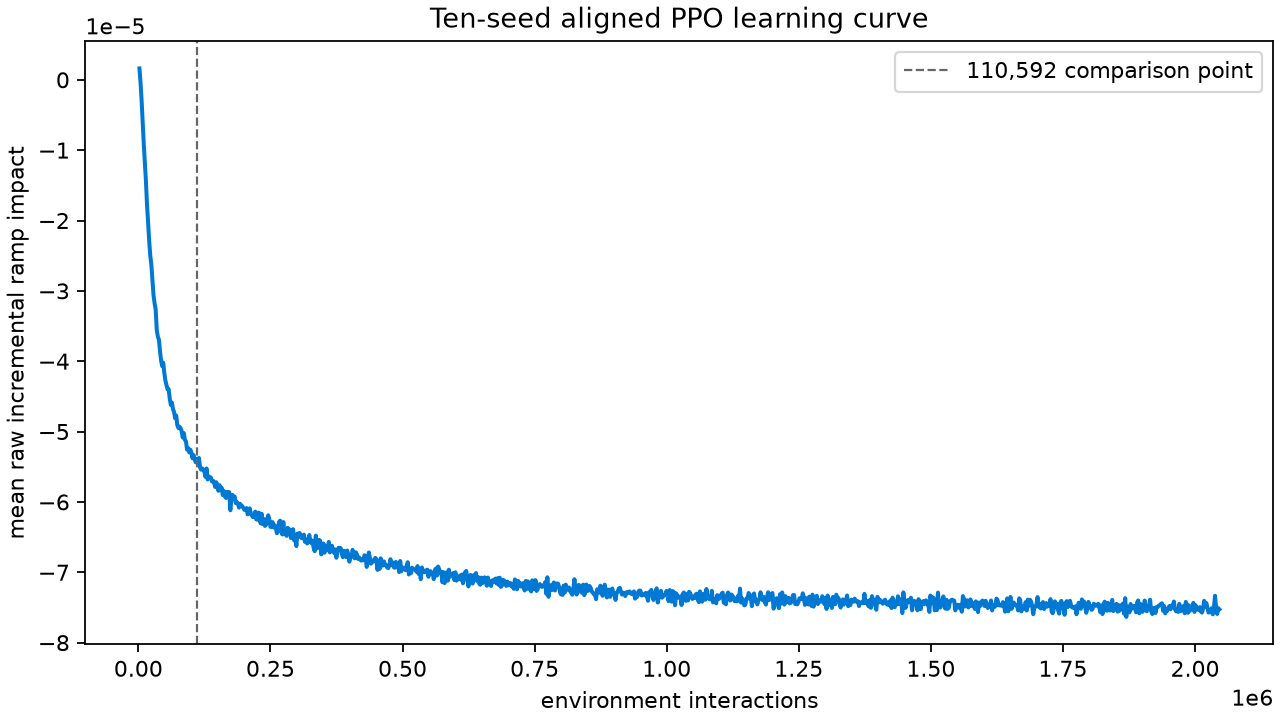
\includegraphics[width=0.90\textwidth]{../output/four_market_v2/campaign/learning_curve_aggregate.png}
  \caption{Ten-seed mean raw incremental ramp impact at each aligned PPO
  rollout. More-negative values are better. The dashed line marks 110,592
  interactions, when learning was still progressing.}
  \label{fig:campaign-learning-curve}
\end{figure}

Over the final 20\% of interactions, the slope remains negative but falls to
\(-1.2654\times10^{-12}\) per interaction, nearly two orders of magnitude
smaller. Training is therefore close to a plateau by 2M interactions, whereas
110,592 interactions was clearly premature. This curve is descriptive and
does not add another significance test.

\subsection{Post-hoc cost and operational safety}
\label{subsec:campaign-cost-safety}

Mean policy day-ahead cost is 1.001233 times status quo, a 0.123\% increase.
Seed ratios range from 0.995687 to 1.007319. Cost is not part of reward and no
budget gate is applied, so this is an outcome rather than a pass/fail result.

Across all ten policies and all 280 policy-validation episodes, service
unserved, unfinished batch, expired batch, terminal work, certificate
violations, and emergency feasibility use are all zero. The macro ramp benefit
was therefore not obtained by dropping work or violating the modeled
constraints.

The compact result is
\codepath{output/four_market_v2/campaign/aggregation.json}; aligned learning
curves are in \codepath{learning_curve_aggregate.csv} and
\codepath{learning_curve_aggregate.png} in the same directory. The executable
entry points are \codepath{scripts/run_four_market_v2_campaign.py} and
\codepath{scripts/aggregate_four_market_v2_campaign.py}.

\begin{thebibliography}{9}
\raggedright

\bibitem{wilkes2020clusterdata2019}
John Wilkes.
\newblock \emph{Google ClusterData2019: Cluster-Usage Traces v3}.
\newblock Public BigQuery trace and documentation, CC BY 4.0, 2020.
\newblock \url{https://github.com/google/cluster-data/blob/master/ClusterData2019.md}.

\bibitem{googleTraceFormatV3}
Google.
\newblock \emph{ClusterData trace format v3}.
\newblock Protocol-buffer schema for the 2019 trace.
\newblock \url{https://github.com/google/cluster-data/blob/master/clusterdata_trace_format_v3.proto}.

\bibitem{googleClusterAnalysisColab}
Google.
\newblock \emph{Google ClusterData2019 analysis Colab}.
\newblock Official BigQuery examples defining the priority bands and top-level
instance filter.
\newblock \url{https://github.com/google/cluster-data/blob/master/clusterdata_analysis_colab.ipynb}.

\bibitem{googlePowerData2019}
Google.
\newblock \emph{PowerData2019: Power-domain traces}.
\newblock Public BigQuery trace and documentation, CC BY 4.0.
\newblock \url{https://github.com/google/cluster-data/blob/master/PowerData2019.md}.

\bibitem{googlePowerAnalysisColab}
Google.
\newblock \emph{Google Data Center Power Trace Analysis}.
\newblock Official PowerData2019 BigQuery analysis notebook.
\newblock \url{https://github.com/google/cluster-data/blob/master/power_trace_analysis_colab.ipynb}.

\bibitem{caisoOasis}
California Independent System Operator.
\newblock \emph{Open Access Same-time Information System (OASIS)}.
\newblock PRC\_LMP v12, TH\_NP15\_GEN-APND.
\newblock \url{https://oasis.caiso.com}.

\bibitem{misoReports}
Midcontinent Independent System Operator.
\newblock \emph{Market Reports}.
\newblock DA ex-post LMP at MINN.HUB.
\newblock \url{https://www.misoenergy.org/markets-and-operations/real-time--market-data/market-reports/}.

\bibitem{sppPublicData}
Southwest Power Pool.
\newblock \emph{Marketplace Public Data: DA-LMP by Settlement Location}.
\newblock SPPNORTH\_HUB.
\newblock \url{https://portal.spp.org/pages/da-lmp-by-settlement-location}.

\bibitem{isoneReports}
ISO New England.
\newblock \emph{Day-Ahead Hourly LMP Reports}.
\newblock WW\_DALMP\_ISO, location 4008.
\newblock \url{https://www.iso-ne.com/isoexpress/web/reports/pricing}.

\bibitem{eiaGridMonitor}
U.S. Energy Information Administration.
\newblock \emph{Hourly Electric Grid Monitor (Form EIA-930)}.
\newblock Includes the EBA.zip bulk archive.
\newblock \url{https://www.eia.gov/electricity/gridmonitor/}.

\end{thebibliography}

\end{document}

% Verification (2026-08-13): 157 active code/data/result claims checked; 151
% confirmed and 6 corrected (none in this result-verification pass). Checked tier
% metrics (8 cells), PowerData coefficients/R2
% (8 cells), Q95 scales (4 markets), the 114/28 calendar, K=1/500 MW geometry,
% raw-arrival maximum 2.4244025972 against capacity four, [2,1,2,3] deadlines,
% the 9-action/100-observation schemas, pure reward, post-hoc cost, and the
% 10-seed campaign: all 10 compact summaries have 2,000,000 requested,
% 2,045,952 effective, resumed_from_interactions=0, and 28 February episodes;
% the aggregation, 999-point CSV/PNG, paired statistics, market results, cost
% range, and zero safety totals agree. Corrections distinguish fixture contents
% from factory panel references, factory construction from preflight validation,
% and modeled warm power from canonical-panel history; they also state the
% absence of Lagrangian, penalty, cost, and separate terminal-tail reward terms.
% No source-manifest hash, workload envelope, deleted data artifact, or campaign
% result is claimed. External-source acquisition history remains cited rather
% than independently revalidated here.
